\chapter{Implementasi dan Pengujian}
\label{chap:implementasi_dan_pengujian}

Bab ini terdiri atas implementasi, pengujian, dan masalah yang dihadapi. Pada bagian implementasi akan dijelaskan mengenai lingkungan implementasi dan hasil dari implementasi. Pada bagian pengujian akan berisi hasil dari pengujian. Pada bagian masalah yang dihadapi akan dijelaskan masalah - masalah yang dihadapi pada saat implementasi.


\section{Implementasi}
\label{sec:implementasi}

\subsection{Lingkungan Implementasi}
\label{sec:lingkungan_implementasi_dan_pengujian}

Berikut adalah spesifikasi \textit{laptop} yang digunakan untuk implementasi:
\begin{enumerate}
    \item \textit{Processor} : AMD Ryzen 7 
    \item \textit{Memory} : 16 GB DDR4 2400MHz SDRAM
    \item \textit{Storage} :  512 GB SSD
    \item \textit{VGA} : NVDIA GTX 1660TI
    \item \textit{OS} : Windows 10 64-bit\\
\end{enumerate}

Berikut adalah spesifikasi \textit{browser} yang digunakan:
\begin{enumerate}
    \item \textit{Name} : Google Chrome  
    \item \textit{Version} : 90.0.4430.212 \\
\end{enumerate}

Berikut adalah spesifikasi perangkat lunak yang digunakan untuk implementasi:
\begin{enumerate}
    \item IDE : Webstrom 2021.1.1
    \item Bahasa Pemrograman : Javascript
    \item \textit{Runtime Enviroment} : node.js 14.17.0 LTS
\end{enumerate}

\subsection{Implementasi Antarmuka Perangkat Lunak}
Pada implementasinya, antarmuka perangkat lunak telah berhasil dirancang sesuai dengan subbab \ref{sec:perancanganAntarmuka}. Berikut adalah hasil implementasinya:

\begin{figure}[H]
	\centering  
	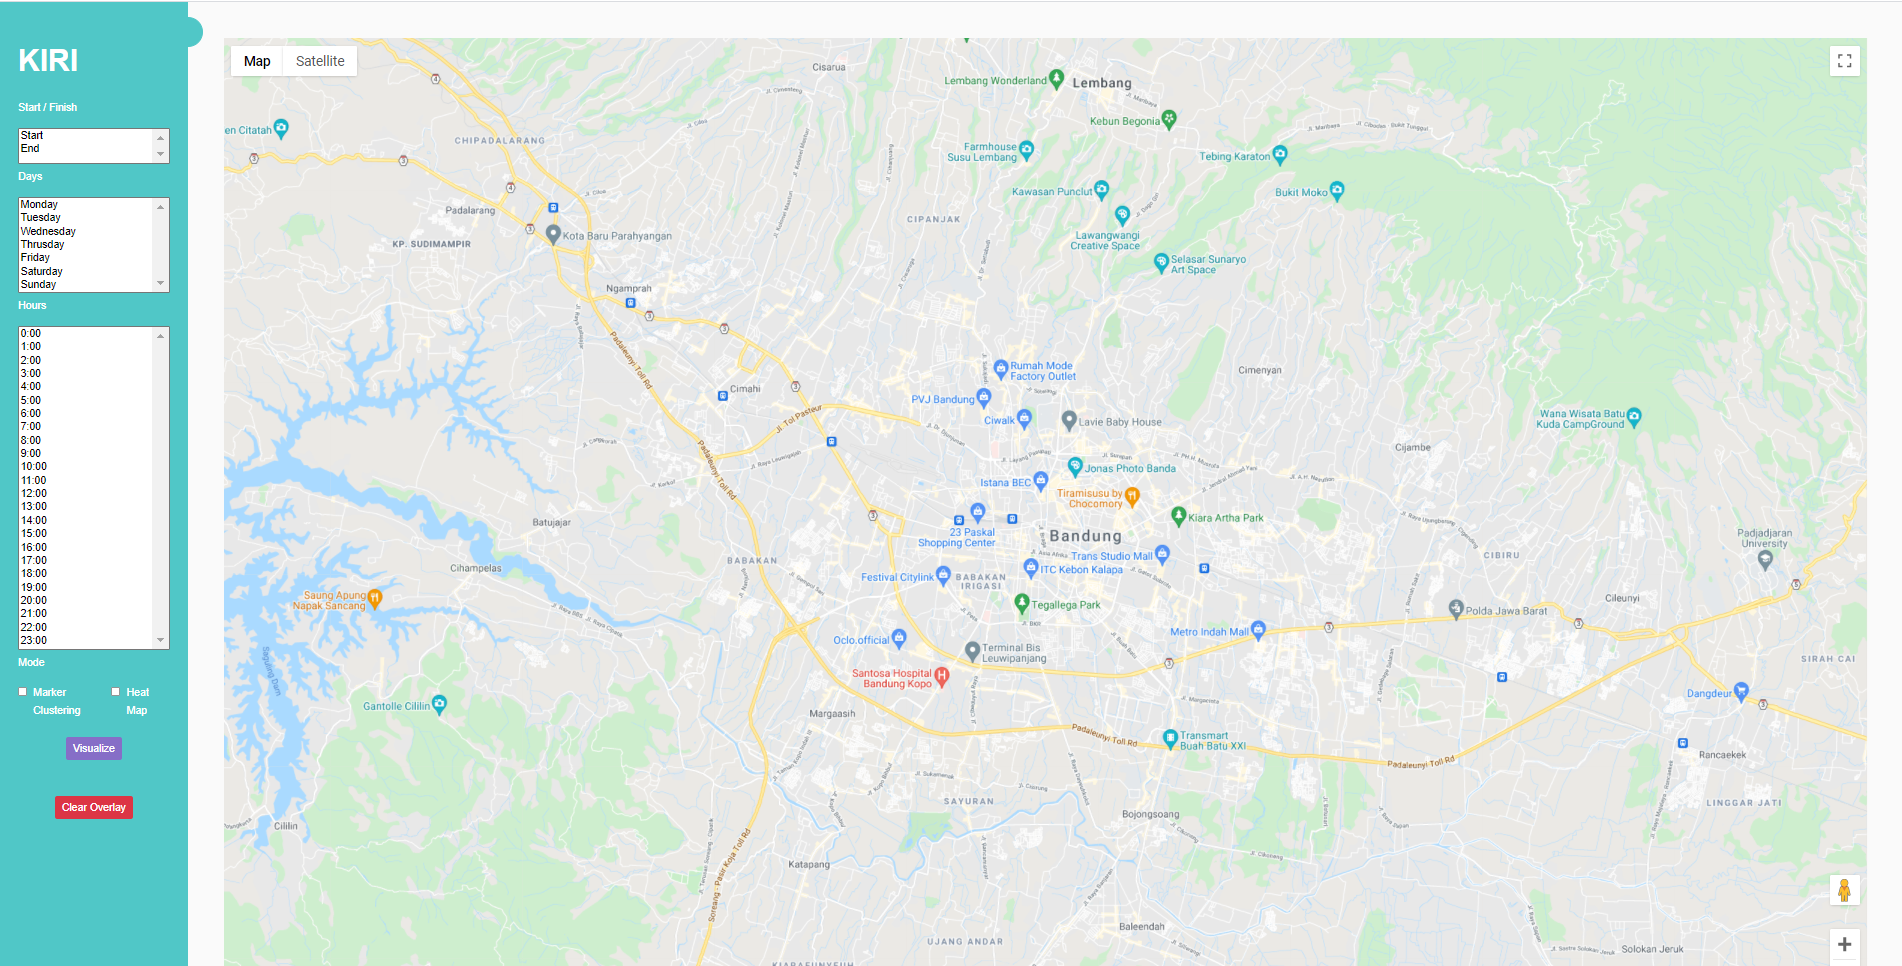
\includegraphics[scale=0.3]{Gambar/Kiri_Ui.PNG}  
	\caption[Tampilan Awal Antarmuka]{Tampilan Awal Antarmuka} 
	\label{fig:interface1} 
\end{figure}

\begin{figure}[H]
	\centering  
	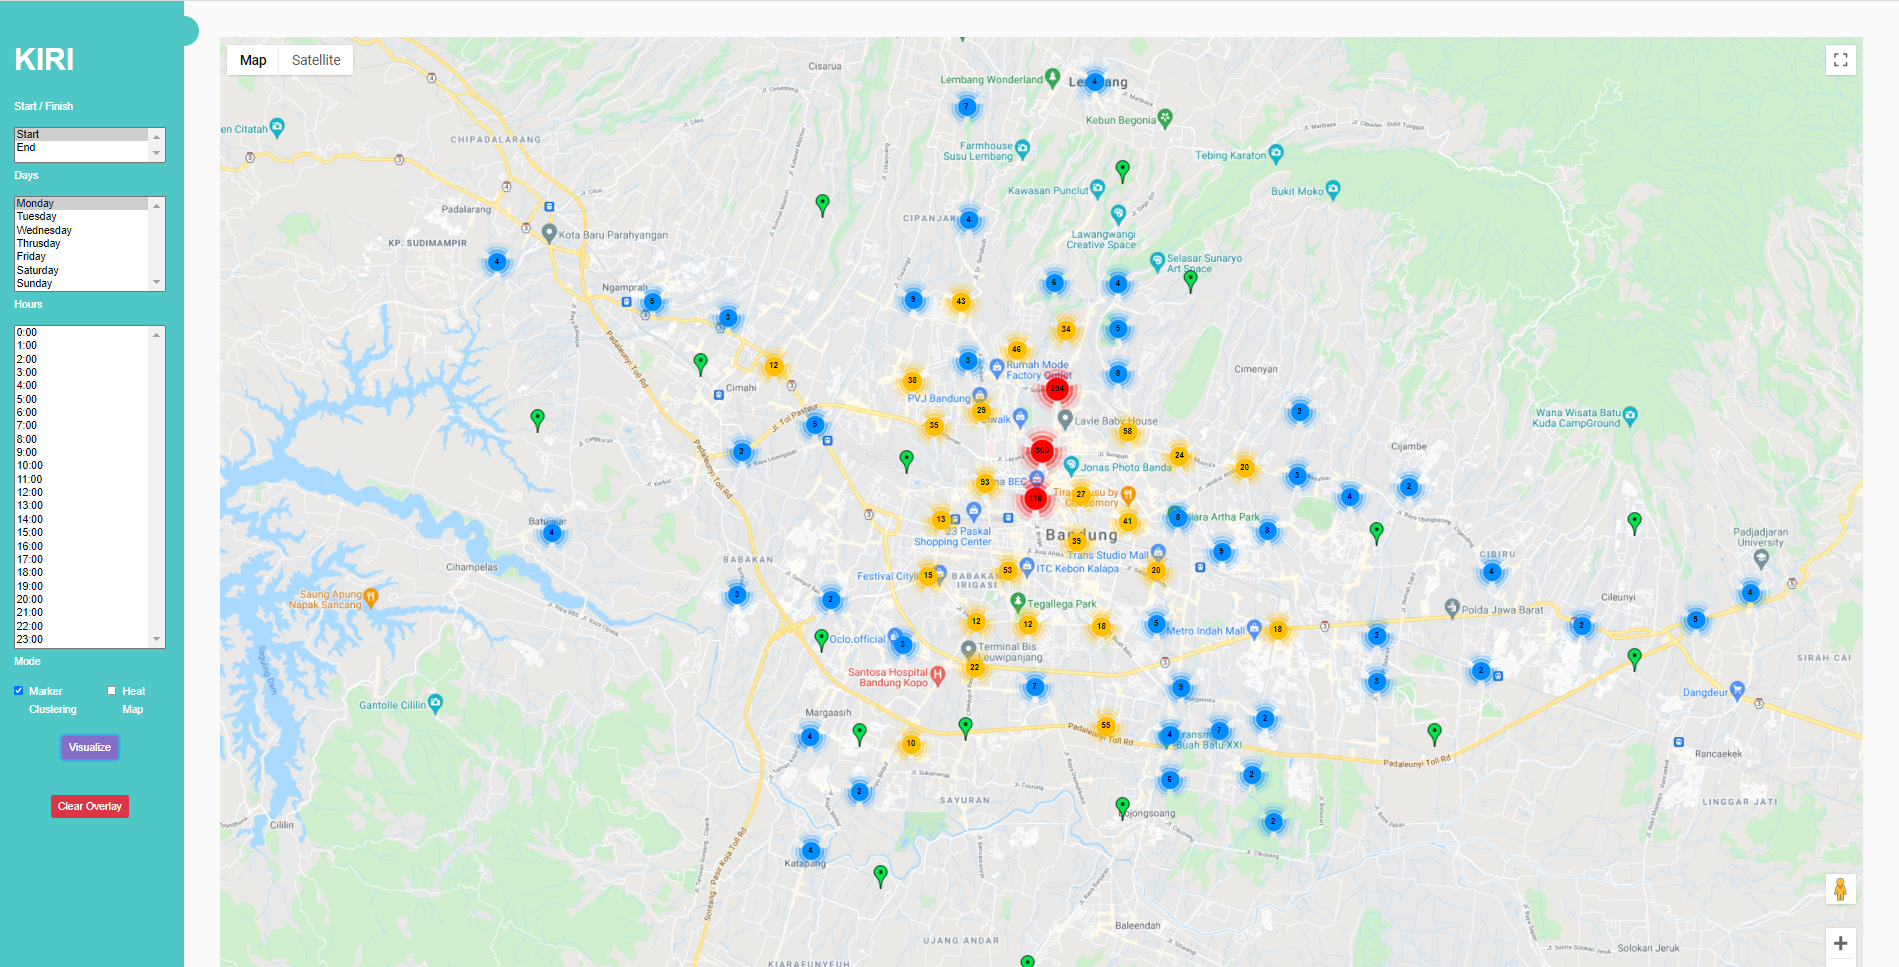
\includegraphics[scale=0.3]{Gambar/Kiri_Ui_Marker.PNG}  
	\caption[Tampilan setelah memilih marker clustering ]{Tampilan setelah memilih marker clustering} 
	\label{fig:interface2} 
\end{figure}

\begin{figure}[H]
	\centering  
	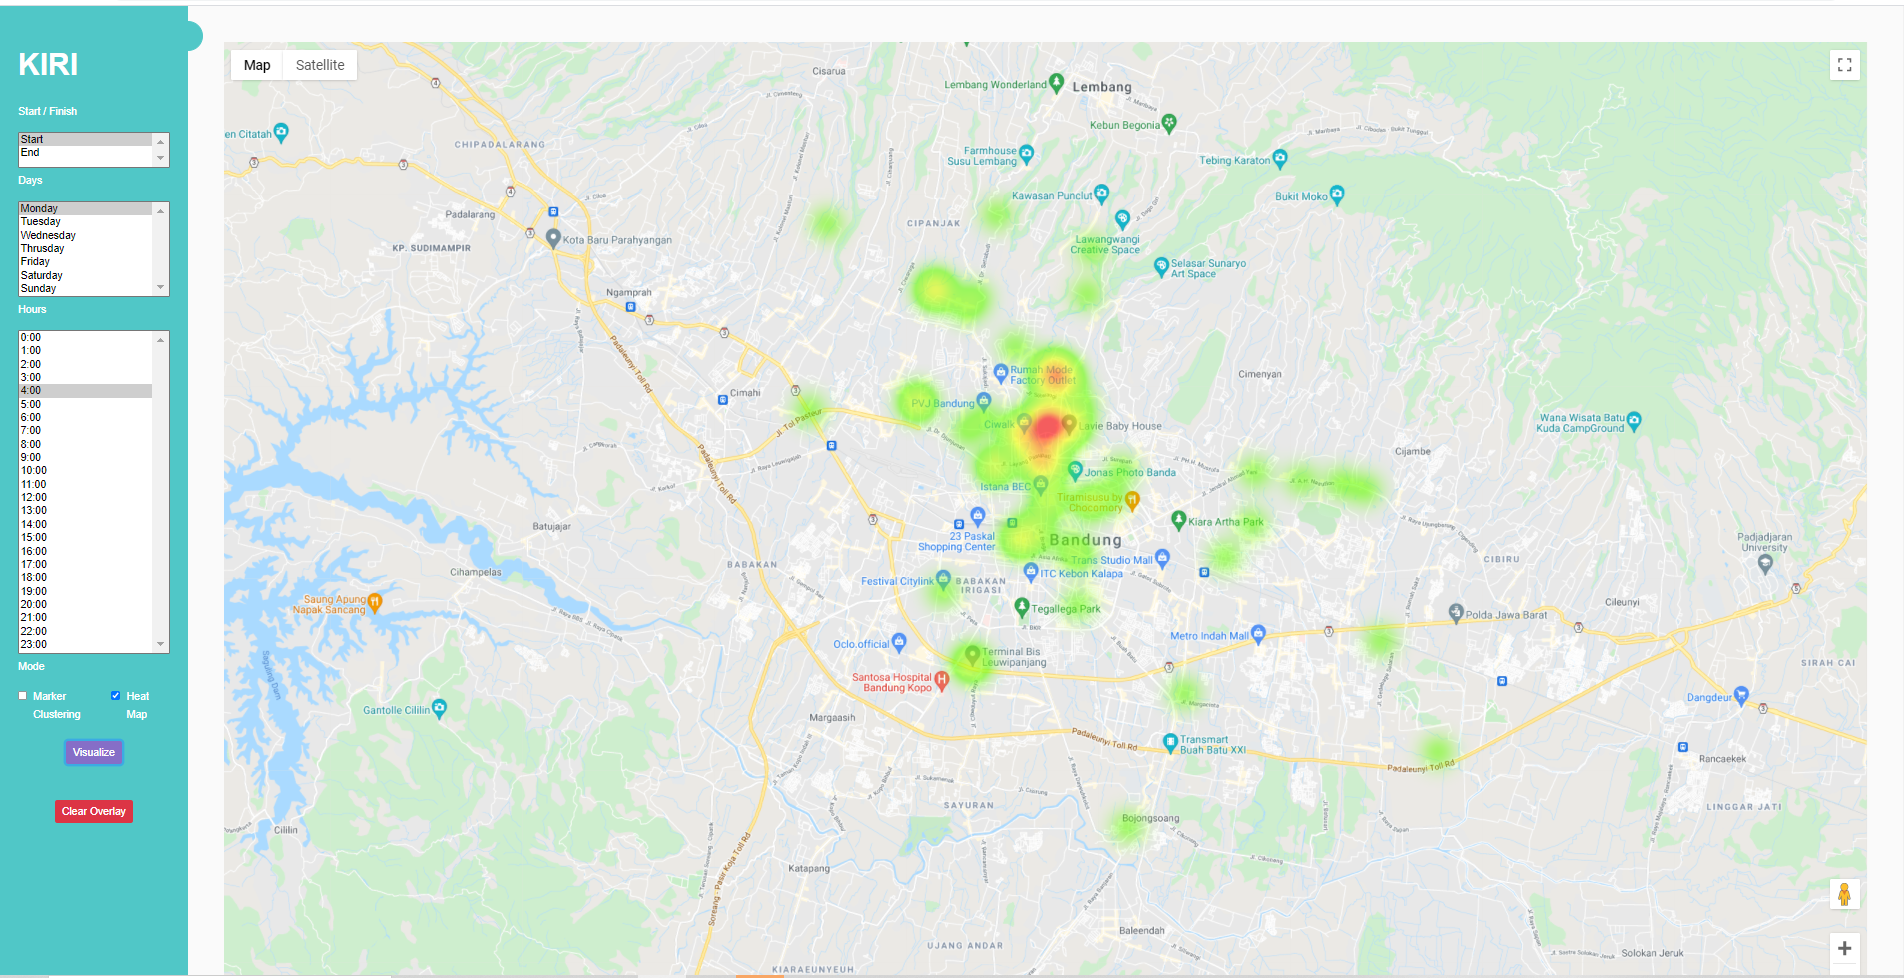
\includegraphics[scale=0.3]{Gambar/Kiri_Ui_Heat_Map.PNG}  
	\caption[Tampilan setelah memilih Heat Map]{Tampilan setelah memilih Heat Map} 
	\label{fig:interface3} 
\end{figure}

\subsection{Implementasi Perangkat Lunak}
Perangkat lunak yang dibuat sesuai dengan perancangan pada Bab \ref{chap:perancangan}. Implementasi aplikasi ini menggunakan bahasa pemrograman Javascript. Terdapat tiga bagian utama dalam perangkat lunak yang dibuat.

\begin{itemize}
    \item \textit{Model} bagian ini adalah representasi dari data, bagian ini juga dapat disebut sebagai \textit{backend}. Pada bagian ini terdapat kelas \textit{model} untuk data histori KIRI. Pada bagian ini juga terdapat kelas \textit{helper} untuk melakukan operasi pengolahan data.
    \item \textit{Router} bagian ini adalah bagian yang menjadi \textit{controller} dalam perangkat lunak. \textit{Router} akan berguna sebagai \textit{media} komunikasi antara \textit{web client} dengan \textit{backend server} 
    \item \textit{View} bagian ini adalah bagian tampilan atau yang bisa disebut \textit{web client} karena pada perangkat lunak ini menggunakan platfrom \textit{website}. Bagian ini bertugas untuk menampilkan hasil visualisasi dan mengolah input dari user.
\end{itemize}

\subsubsection{Model}
Bagian ini adalah representasi dari data, bagian ini juga dapat disebut sebagai \textit{backend}. Pada bagian ini terdapat kelas \textit{model} untuk data histori KIRI. Pada bagian ini juga terdapat kelas \textit{helper} untuk melakukan operasi pengolahan data. Berikut ini adalah gambaran kelas \textit{model} data histori KIRI:

\newpage \begin{lstlisting}[label=Kiri_Model, language=JavaScript, caption=Metode Load Data, breaklines]
const fs = require("fs")
const {csvToObject, buildFilter, filterData} = require("./Utils");

class KiriHistory {
    constructor() {
        fs.readFile(__dirname + "/data/KIRIStatistics.csv", "utf8", ((err, data) => {
            if (err === null) {
                let arrCSV = data.split("\n")
                arrCSV.shift();
                this.data = arrCSV.map(csvToObject).filter(item => item !== undefined);
            }
        }))
    }

    //return promise
    getData = (filterParams) => {
        let query = buildFilter(filterParams);
        this.data = filterData(this.data, query);
        return this.data;
    }

}

module.exports = KiriHistory;

\end{lstlisting}

Pada kelas model ini memiliki dua action utama yaitu:
\subsubsection{Load Data}
Action ini akan dijalankan begitu objek \textit{model} dibuat. Action ini akan melakukan load dan normalisasi data histori kiri. Action ini akan menggunakan method \textit{readFile} yang berasal dari \textit{package filesystem}. Berikut ini adalah contoh implementasi dari action ini.


\begin{lstlisting}[label=Kiri_Model, language=JavaScript, caption=Metode Load Data, breaklines]
constructor() {
fs.readFile(__dirname + "/data/KIRIStatistics.csv", "utf8", ((err, data) => {
    if (err === null) {
        let arrCSV = data.split("\n")
        arrCSV.shift();
        this.data = arrCSV.map(csvToObject).filter(item => item !== undefined);
    }
    }))
}
\end{lstlisting}


Method \textit{reafFile} akan melakukan action load pada data histori KIRI \ref{sec:analisisDataHistoriKiri}. Data yang akan diload bertipe \textit{csv} dan memiliki format data sebagai berikut.
\begin{lstlisting}[label=Kiri_Histori_Data, caption=Histori Data KIRI]
logId,APIKey,Timestamp (UTC),Action,AdditionalData
113909,E5D9904F0A8B4F99,2/1/2014 0:07,PAGELOAD,/5.10.83.30/
113914,A44EB361A179A49E,2/1/2014 0:11,SEARCHPLACE,taman+fot/10
113915,A44EB361A179A49E,2/1/2014 0:11,FINDROUTE,"-6.8972513,107.6385574/-6.91358,107.62718/1"
114256,308201BB30820124,2/1/2014 5:24,SEARCHPLACE,soekarno+hatta+643/10
\end{lstlisting}
Ketika \textit{readFile} dijalankan \textit{fungsi} ini akan memiliki \textit{callback} yang akan mengembalikan data histori kiri, data yang telah diload oleh \textit{readFile} akan berbentuk seperti: 
\begin{lstlisting}[label=load_data_1 , caption=Raw Data]
[
 'logId,APIKey,Timestamp (UTC),Action,AdditionalData\r',
  '113909,E5D9904F0A8B4F99,2/1/2014 0:07,PAGELOAD,/5.10.83.30/\r',
  '113910,E5D9904F0A8B4F99,2/1/2014 0:07,PAGELOAD,/5.10.83.49/\r',
  '113911,E5D9904F0A8B4F99,2/1/2014 0:09,PAGELOAD,/5.10.83.30/\r',
]
\end{lstlisting}
Data tersebut akan ditampung ke dalam variable yang diberinama \textit{arrCSV}. Baris pertama dari data ini adalah \textit{header} dari csv. Pada proses normalisasi data baris pertama ini tidaklah dibutuhkan oleh karena itu akan dihilangkan baris pertama menggunakan method \textit{shift()}. Sehingga data akan berbentuk:
\begin{lstlisting}[label=load_data_2 , caption=Raw Data 2]
[
  '113909,E5D9904F0A8B4F99,2/1/2014 0:07,PAGELOAD,/5.10.83.30/\r',
  '113910,E5D9904F0A8B4F99,2/1/2014 0:07,PAGELOAD,/5.10.83.49/\r',
  '113911,E5D9904F0A8B4F99,2/1/2014 0:09,PAGELOAD,/5.10.83.30/\r',
]
\end{lstlisting}
Data tersebut kemudian akan dipetakan ke dalam \textit{map} dengan menggunakan fungsi mapper yang diberi nama \textit{csvToObject}. Fungsi ini akan memetakan dan melakukan \textit{formating} dari setiap value dari \ref{load_data_2}.

\begin{lstlisting}[label=helper_1 , caption=CSV Mapper]
const csvToObject = item => {
    let cols = item.split(",")
    let action = cols[3];
    if (action === "FINDROUTE") {
        let startLng = cols[5].split("/")[0]
        let endLat = cols[5].split("/")[1]
        let fullDate = new Date(cols[2])
        return {
            apiKey: cols[0],
            timestamp: fullDate,
            action,
            startCor: {lat: parseFloat(cols[4].substr(1)), lng: parseFloat(startLng)},
            endCor: {lat: parseFloat(endLat), lng: parseFloat(cols[6].split("/")[0])},
            day: fullDate.getDay(),
            hour: fullDate.getHours()
        }
    }
}
\end{lstlisting}

Fungsi ini akan akan memanfaatkan \textit{method split} untuk membagi raw data \ref{load_data_2} menjadi array yang berbentuk:

\begin{lstlisting}[label=data_parser_1 , caption=Data Split Result]
[
  '115566',
  'A44EB361A179A49E',
  '2/2/2014 9:07',
  'FINDROUTE',
  '"-0.7819376',
  '100.2871169/-6.90359',
  '107.60040/1"\r'
]

\end{lstlisting}
Berdasarkan data \ref{data_parser_1} kita dapat mengekstrak  \textit{action type} \ref{sec:analisisDataHistoriKiri} pada posisi ketiga dari array tersebut. Dalam aplikasi ini hanya akan digunakan data yang memiliki action \textit{FINDROUTE} hal ini dikarenakan hanya pada \textit{action} ini data menggandung value dari posisi start dan finish. Setelah function \textit{csvToObject} ini dijalankan maka akan mengembalikan kumpulan objek data yang berbentuk:

\begin{lstlisting}[label=data_parser_result , caption=Result Data]
[
    {
      apiKey: '113915',
      timestamp: 2014-01-31T17:11:00.000Z,
      action: 'FINDROUTE',
      startCor: { lat: -6.8972513, lng: 107.6385574 },
      endCor: { lat: -6.91358, lng: 107.62718 },
      day: 6,
      hour: 0
    }
]
\end{lstlisting}

\subsubsection{Get Data}
Fungsi ini akan dijalankan setiap ada request dari \textit{web client}. Action ini akan mengembalikan data histori KIRI sesuai dengan filter parameter yang diberikan. Berikut ini adalah contoh implementasi dari action ini:
\begin{lstlisting}[label=get_data , caption=Function Get Data]
    getData = (filterParams) => {
        let query = buildFilter(filterParams);
        this.data = filterData(this.data, query);
        return this.data;
    }
\end{lstlisting}
Pada fungsi ini akan menerima paramter \textit{filterParams} yang berasal dari \textit{web client}. Fungsi ini akan menjalankan dua perintah yaitu \textit{buildFilter} dan  \textit{filterData} dan akan mengembalikan data histori yang sesuai dengan filterParams yang diberikan. Fungsi \textit{buildFilter} akan mengubah filterParams  yang berbentuk:
\begin{lstlisting}[label=filter_params , caption=Filter Parameter]
{
    day: [ 0 ], 
    hour: [ 8, 9, 10, 11 ] 
}
\end{lstlisting}
Menjadi \textit{query params}. Hal ini dilakukan karena fungsi \textit{filter} yang dirancang pada perangkat lunak ini akan memanfaatkan \textit{function} filter dari javascript.

\newpage 
\subsubsection{Filter Data}
 Berikut ini adalah hasil implementasi dari function filter:
\begin{lstlisting}[label=filter_method , caption=Fungsi Filter]
 const filterData = (data, query) => {
    const keysWithMinMax = [];
    const filteredData = data.filter((item) => {
        for (let key in query) {
            if (item[key] === undefined) {
                return false;
            } else if (keysWithMinMax.includes(key)) {
                if (query[key]['min'] !== null && item[key] < query[key]['min']) {
                    return false;
                }
                if (query[key]['max'] !== null && item[key] > query[key]['max']) {
                    return false;
                }
            } else if (!query[key].includes(item[key])) {
                return false;
            }
        }
        return true;
    });
    return filteredData;
};
\end{lstlisting}

Fungsi ini akan memanfaatkan \textit{method filter dan includes javascript}. Fungsi ini akan menghasilkan data yang telah disaring sesuai dengan query params yang diberikan.


\subsection{Router}
Bagian ini merupakan bagian yang bertugas sebagai \textit{controller} antara \textit{backend logic} dan \textit{web client}. Implementasi router dapat dilihat sebagai berikut:
\begin{lstlisting}[label=Router , caption=Router Implementation]
const express = require('express')
const app = express()
const Kiri = require("../model/Kirihistory");
const path = require('path');
const viewPath = "C:/KiriHistory/views"
let modelKiri = new Kiri();
app.use(express.json())
app.get("/", (req, res) => {
    res.sendFile(path.join(`${viewPath}/index.html`));
})


app.post('/searchRoute', (req, res) => {
    let filterParams = req.body;
    let data = modelKiri.getData(filterParams);
    res.status(200).json({
        'status': 'OK',
        'messages': 'Data',
        'data': data,
    })

})
module.exports = {app, express};
\end{lstlisting}
Bagian ini memiliki dua fungsi utama yaitu melakukan render untuk \textit{web client} dan mengatur \textit{response} dan \textit{request} antara \textit{web client} dan \textit{backend logic}.

\subsubsection{Redner HTML}
Perangkat lunak ini menggunakan \textit{node.js} sebagai \textit{runtime manager}. Perangkat lunak ini memanfaatkan method \textit{sendFile} milik \textit{node.js} untuk dapat melakukan \textit{rendering} pada \textit{route} yang diinginkan. Implementasi pada bagian ini dapat dilhat sebagai berikut:

\begin{lstlisting}[label=render_html , caption=Render HTML]
app.get("/", (req, res) => {
    res.sendFile(path.join(`${viewPath}/index.html`));
})
\end{lstlisting}
Pada potongan kode diatas menunjukan bahwa \textit{index.html} akan dirender pada \textit{route '/'}.

\subsection{Controller antara \textit{Web client} dan \textit{Backend Logic}}
Implementasi pada bagian ini dapat dilhat sebagai berikut:
\begin{lstlisting}[label=render_html , caption=Render HTML]
app.post('/searchRoute', (req, res) => {
    let filterParams = req.body;
    let data = modelKiri.getData(filterParams);
    res.status(200).json({
        'status': 'OK',
        'messages': 'Data',
        'data': data,
    })

})
\end{lstlisting}

Pada bagian ini perangkat lunak akan membuat \textit{endpoint} yang akan menerima parameter berupa \textit{filter parameter} dan akan mengembalikan hasil data histori yang telah di filter.

\subsubsection{View}
Bagian ini adalah bagian disebut \textit{web client} \ref{sec:webclientCapability}. Pada bagian ini terdapat fungsi untuk menerima \textit{input user} dan menampilkan hasil visualisasi menggunakan \textit{Google Maps Javascript API}. Pada bagian ini format \textit{user interface} akan ditulis dalam  format \textit{Hypertext Markup Language (html)} hal ini dapat dilihat pada file \textit{index.html}.
Selain untuk tampilan bagian ini juga berfungsi untuk menerima input user dan mengubahnya menjadi \textit{filter params}, hal ini dapat dilihat pada file \textit{maps.js}. Bentuk implementasi dari bagian ini dapat dilihat:

\begin{lstlisting}[label=maps_js , caption=Maps.js]
function initMap() {
    let map = new google.maps.Map(document.getElementById("map"), {
        center: {lat: -6.914744, lng: 107.609810},
        zoom: 13,

    });
    return map;
}

function setMarkers(data, isStart, isEnd) {
    let locations = [];
    if (isStart) {
        data.forEach(item => {
            let startMark = {
                name: "start",
                pos: item.startCor,
                icon: "http://maps.google.com/mapfiles/ms/icons/green-dot.png"
            }
            locations.push(startMark)
        })
    }

    if (isEnd) {
        data.forEach(item => {
            let endMark = {name: "end", pos: item.endCor, icon: "http://maps.google.com/mapfiles/ms/icons/red-dot.png"}
            locations.push(endMark)
        })
    }

    // console.log("filtered markers size" , data.length)
    let markers = locations.map((item) => {
        return new google.maps.Marker({
            position: {lat: parseFloat(item.pos.lat), lng: parseFloat(item.pos.lng)},
            icon: item.icon
        });
    });
    return markers;
}

function setHeatMap(arrData, map, isStart, isEnd) {
    let heatmapData = [];
    if (isStart) {
        arrData.forEach(item => {

            let startCoor = {location: new google.maps.LatLng(item.startCor.lat, item.startCor.lng)}
            heatmapData.push(startCoor)

        })
    }
    if (isEnd) {
        arrData.forEach(item => {
            // {location: new google.maps.LatLng(37.782, -122.447), weight: 0.5},
            let endLocationObj = {location: new google.maps.LatLng(item.endCor.lat, item.endCor.lng)}
            heatmapData.push(endLocationObj)
        })
    }

    let heatmap = new google.maps.visualization.HeatmapLayer({
        data: heatmapData,
        radius: 50
    });
    heatmap.setMap(map);

    return heatmap;
}

function sendRequest(url, data = {}) {
    return axios.post(url, data);
}


function docReady(fn) {
    // see if DOM is already available
    if (document.readyState === "complete" || document.readyState === "interactive") {
        // call on next available tick
        setTimeout(fn, 1);
    } else {
        document.addEventListener("DOMContentLoaded", fn);
    }
}


createFilterObj = () => {
    let days = Array.from(document.getElementById("day").selectedOptions).map(option => parseInt(option.value))
    let hours = Array.from(document.getElementById("hour").selectedOptions).map(option => parseInt(option.value));
    let filter = {day: days, hour: hours}
    return filter
}


deleteMarkes = (markers) => {
    markers.forEach(item => {
        item.setMap(null)
    })
    return null
}


docReady(function () {
    let map = initMap()
    let markerCluster = null;
    let markers;
    let heatMap;
    document.getElementById("send-btn").onclick = function (e) {
        e.preventDefault();
        let filterParams = createFilterObj()
        let isMarkerCluster = document.getElementById("marker-cluster").checked
        let isHeatMap = document.getElementById("heat-map").checked
        let statusSelected = Array.from(document.getElementById("start-finish").selectedOptions).map(option => option.value)
        let statusStartChecked = statusSelected.includes("start");
        let statusEndChecked = statusSelected.includes("end")
        sendRequest("http://localhost:3000/searchRoute", filterParams).then(res => {
            if (isMarkerCluster) {
                map.setMapTypeId(google.maps.MapTypeId.ROADMAP);
                let data = res.data.data;
                if (!Array.isArray(markers)) {
                    markers = setMarkers(data, statusStartChecked, statusEndChecked)
                    markerCluster = new MarkerClusterer(map, markers, {
                        imagePath:
                            "https://developers.google.com/maps/documentation/javascript/examples/markerclusterer/m",
                    });
                }
            }

            if (isHeatMap) {
                map.setMapTypeId(google.maps.MapTypeId.ROADMAP);
                if (!heatMap || heatMap.getMap() === null) {
                    heatMap = setHeatMap(res.data.data, map, statusStartChecked, statusEndChecked)
                }
            }
        });
    }

    document.getElementById('clear-btn').onclick = function (e) {
        e.preventDefault();
        if (markerCluster) {
            markerCluster.removeMarkers(markers);
            markers = deleteMarkes(markers)
        }
        if (heatMap) {
            heatMap.setMap(null)
        }
    }
});


\end{lstlisting}

Bagian ini memiliki tiga tugas utama yaitu:
\begin{itemize}
    \item Menerina input user dan mengubah input user menjadi \textit{filter params}.
    \item Mengirim dan menerima data dari \textit{router}.
    \item Membuat google maps input dan berkomunikasi dengan \textit{google maps javascript api}.
\end{itemize}

\subsubsection{ Menerina input user dan mengubah input user menjadi \textit{filter params}}
Implementasi bagian ini dapat dilihat menjadi:
\begin{lstlisting}[label=input_user , caption=Input User]
createFilterObj = () => {
    let days = Array.from(document.getElementById("day").selectedOptions).map(option => parseInt(option.value))
    let hours = Array.from(document.getElementById("hour").selectedOptions).map(option => parseInt(option.value));
    let filter = {day: days, hour: hours}
    return filter
}

\end{lstlisting}

Ketika fungsi ini dijalankan maka akan mengambil value dari element dengan id \textit{day} dan \textit{hour}. Kemudian data tersebut akan dibuat ke dalam bentuk \textit{map} yang disebut sebagai \textit{filter parameter}. Pada bagian ini juga terdapat fungsi \textit{docReady} yang bertugas untuk  berkomunikasi dengan \textit{node.js} atau \textit{google maps javascript api}. Hasil implementasi fungsi tersebut adalah sebagai berikut:
\begin{lstlisting}[label=docReady , caption=docReady Method]
function docReady(fn) {
    if (document.readyState === "complete" || document.readyState === "interactive") {
        setTimeout(fn, 1);
    } else {
        document.addEventListener("DOMContentLoaded", fn);
    }
}

\end{lstlisting}
Pada fungsi ini memiliki parameter sebuah fungsi dimana fungsi ini akan dijalankan setiap \textit{tick}. Hal ini dilakukan agar koneksi antar \textit{backend} bisa tetap terus dilakukan. Berikut ini implementasi fungsi \textit{docReady} pada perangkat lunak ini:

\newpage
\begin{lstlisting}[label=docReady_1 , caption=docReady Method]
docReady(function () {
    let map = initMap()
    let markerCluster = null;
    let markers;
    let heatMap;
    document.getElementById("send-btn").onclick = function (e) {
        e.preventDefault();
        let filterParams = createFilterObj()
        let isMarkerCluster = document.getElementById("marker-cluster").checked
        let isHeatMap = document.getElementById("heat-map").checked
        let statusSelected = Array.from(document.getElementById("start-finish").selectedOptions).map(option => option.value)
        let statusStartChecked = statusSelected.includes("start");
        let statusEndChecked = statusSelected.includes("end")
        sendRequest("http://localhost:3000/searchRoute", filterParams).then(res => {
            if (isMarkerCluster) {
                map.setMapTypeId(google.maps.MapTypeId.ROADMAP);
                let data = res.data.data;
                if (!Array.isArray(markers)) {
                    markers = setMarkers(data, statusStartChecked, statusEndChecked)
                    markerCluster = new MarkerClusterer(map, markers, {
                        imagePath:
                            "https://developers.google.com/maps/documentation/javascript/examples/markerclusterer/m",
                    });
                }
            }

            if (isHeatMap) {
                map.setMapTypeId(google.maps.MapTypeId.ROADMAP);
                if (!heatMap || heatMap.getMap() === null) {
                    heatMap = setHeatMap(res.data.data, map, statusStartChecked, statusEndChecked)
                }
            }
        });
    }

    document.getElementById('clear-btn').onclick = function (e) {
        e.preventDefault();
        if (markerCluster) {
            markerCluster.removeMarkers(markers);
            markers = deleteMarkes(markers)
        }
        if (heatMap) {
            heatMap.setMap(null)
        }
    }
});

\end{lstlisting}

\newpage \subsubsection{Mengirim dan menerima data dari router}
Implementasi untuk bagian ini dapat dilihat pada method docReady:

\begin{lstlisting}[label=communication , caption=communication method]
    document.getElementById("send-btn").onclick = function (e) {
        e.preventDefault();
        let filterParams = createFilterObj()
        let isMarkerCluster = document.getElementById("marker-cluster").checked
        let isHeatMap = document.getElementById("heat-map").checked
        let statusSelected = Array.from(document.getElementById("start-finish").selectedOptions).map(option => option.value)
        let statusStartChecked = statusSelected.includes("start");
        let statusEndChecked = statusSelected.includes("end")
        sendRequest("http://localhost:3000/searchRoute", filterParams).then(res => {
            if (isMarkerCluster) {
                map.setMapTypeId(google.maps.MapTypeId.ROADMAP);
                let data = res.data.data;
                if (!Array.isArray(markers)) {
                    markers = setMarkers(data, statusStartChecked, statusEndChecked)
                    markerCluster = new MarkerClusterer(map, markers, {
                        imagePath:
                            "https://developers.google.com/maps/documentation/javascript/examples/markerclusterer/m",
                    });
                }
            }

            if (isHeatMap) {
                map.setMapTypeId(google.maps.MapTypeId.ROADMAP);
                if (!heatMap || heatMap.getMap() === null) {
                    heatMap = setHeatMap(res.data.data, map, statusStartChecked, statusEndChecked)
                }
            }
        });
    }
\end{lstlisting}

Pada potongan kode diatas dapat dilihat jika tombol send-btn ditekan maka akan memanggil method \textit{sendRequest} method ini akan bertujuan untuk berkomunikasi dengan \textit{backend} untuk mendapatkan data yang histori yang telah disaring berdasarkan input dari user. Fungsi ini juga bertujuan untuk mendapatkan hasil visualisasi dari data yang telah disaring dengan menggunakan \textit{google maps javascript api}.

\subsection{Berkomunikasi dengan \textit{google maps javascript api}}
Perangkat lunak ini menggunakan \textit{google maps javasript api} sebagai salah satu \textit{thrid party library} untuk melakukan visualisasi data. Terdapat dua buah opsi yang disediakan oleh perangkat lunak ini dalam melakukan visualisasi data yaitu \textit{Heat Map} dan \textit{Marker Clustering}. Untuk dapat menggunakan opsi tersebut \textit{web client} perlu membuat input parameter yang sesuai dengan kebutuhan \textit{google maps javascript api} \ref{sec:googlemaps}. Implementasi dari bagian ini dapat dilihat sebagai berikut:

\begin{lstlisting}[label=map_input , caption=Map Input]
function setMarkers(data, isStart, isEnd) {
    let locations = [];
    if (isStart) {
        data.forEach(item => {
            let startMark = {
                name: "start",
                pos: item.startCor,
                icon: "http://maps.google.com/mapfiles/ms/icons/green-dot.png"
            }
            locations.push(startMark)
        })
    }

    if (isEnd) {
        data.forEach(item => {
            let endMark = {name: "end", pos: item.endCor, icon: "http://maps.google.com/mapfiles/ms/icons/red-dot.png"}
            locations.push(endMark)
        })
    }

    // console.log("filtered markers size" , data.length)
    let markers = locations.map((item) => {
        return new google.maps.Marker({
            position: {lat: parseFloat(item.pos.lat), lng: parseFloat(item.pos.lng)},
            icon: item.icon
        });
    });
    return markers;
}


function setHeatMap(arrData, map, isStart, isEnd) {
    let heatmapData = [];
    if (isStart) {
        arrData.forEach(item => {

            let startCoor = {location: new google.maps.LatLng(item.startCor.lat, item.startCor.lng)}
            heatmapData.push(startCoor)

        })
    }
    if (isEnd) {
        arrData.forEach(item => {
            // {location: new google.maps.LatLng(37.782, -122.447), weight: 0.5},
            let endLocationObj = {location: new google.maps.LatLng(item.endCor.lat, item.endCor.lng)}
            heatmapData.push(endLocationObj)
        })
    }

    let heatmap = new google.maps.visualization.HeatmapLayer({
        data: heatmapData,
        radius: 50
    });
    heatmap.setMap(map);

    return heatmap;
}

\end{lstlisting}